\documentclass[11pt]{article}
\usepackage{amsmath}
\usepackage{tikz}
\date{\today}
\title{}
\begin{document}

\section{Network equations}

\subsection{Single neuron}

Network representation

\begin{center}
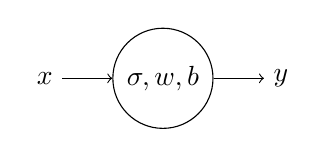
\begin{tikzpicture}
  \def\d{1.5}
  \node (X) at (-\d, 0) {$x$};
  \node[shape=circle, draw=black] (N) at (0, 0) {$\sigma, w, b$};
  \node (Y) at (\d, 0) {$y$};
  \path[->] (X) edge (N);
  \path[->] (N) edge (Y);
\end{tikzpicture}
\end{center}

Forwarding equation

\begin{equation}
  y = \sigma(w x + b)
\end{equation}

Cost function

\begin{equation}
  c(w, b) = \sum_{i=1}^{N} (\sigma(w x_{i} + b) - y_{i})^{2}
\end{equation}

where the error of the forwaring is
\begin{equation}
  \epsilon(x_{i}) = \epsilon_{i} = (\sigma(w x_{i} + b) - y_{i})
\end{equation}

Cost function derivatives

\begin{align}
  \frac{\partial c}{\partial w} &= \sum_{i=1}^{N} 2x_{i}(\sigma(w x_{i} + b) - y_{i})(1 - \sigma(w x_{i} + b))
  = \sum_{i=1}^{N} 2x_{i}(y(x_{i}) - y_{i})(1 - y(x_{i})) = \sum_{i=1}^{N} 2x_{i}\epsilon_{i}(1-y_{i}) \\
  \frac{\partial c}{\partial b} &= \sum_{i=1}^{N} 2(\sigma(w x_{i} + b) - y_{i})(1 - \sigma(w x_{i} + b))
  = \sum_{i=1}^{N} 2(y(x_{i}) - y_{i})(1 - y(x_{i})) = \sum_{i=1}^{N} 2\epsilon_{i}(1-y_{i})
\end{align}
\end{document}
